\documentclass[11pt,a4paper]{article}
\usepackage[margin=1in]{geometry}
\usepackage{hyperref}
\usepackage{enumitem}
\usepackage{graphicx}
\usepackage{xcolor}

% -----------------------------------------------------
% bvraghav-tiet-ucs503p-article.sty
% -----------------------------------------------------

% Variable: Lab Instructor
\makeatletter \newcommand{\BvrSetLabInstructor}[1]{%
  \gdef\Bvr@LabInstructor{#1}}
% default
\newcommand{\Bvr@LabInstructor}{Jhonsy Bansal}
% public accessor
\newcommand{\BvrLabInstructorValue}{\Bvr@LabInstructor}
\makeatother

% Add subtitle
\usepackage{titling}
% -- Set title bold
\pretitle{\begin{center}\bfseries\fontsize{18bp}{18bp}\selectfont}
\makeatletter
\newcommand{\BvrSubtitle}[1]{%
  \posttitle{%
    \par\end{center}
    \begin{center}\large#1\end{center}
    \vskip 0.5em}%
}
\makeatother

\usepackage{tikz}
\usetikzlibrary{positioning, arrows.meta, shapes.geometric}

\usepackage{titlesec}

\titlespacing*{\section}
{0pt}{1.2em}{0.5em}

\titlespacing*{\subsection}
{0pt}{0.8em}{0.4em}

% Hints in the section title(s)
\newcommand{\BvrHint}[1]{%
  {\normalfont\normalsize\itshape\hfill #1}}

% -----------------------------------------------------

\title{NexusLB: A Custom Reverse Proxy \& Load Balancer}

\BvrSetLabInstructor{Jhonsy Bansal}

\BvrSubtitle{%
  Project Proposal for UCS503P  \\
  Submitted to: \BvrLabInstructorValue \\ \bfseries
  Thapar Institute of Engineering and Technology% 
}

\author{
  Navjot Singh, CSED%
  \thanks{Roll No: \texttt{1024030313}, %
    Email: \texttt{nsingh2\_be24\@thapar.edu}}
  \and 
  Shaina Gera, CSED%
  \thanks{Roll No: \texttt{1024030316}, %
    Email: \texttt{sgera\_be24\@thapar.edu}}
  \and 
  Prabhgun Kaur, CSED%
  \thanks{Roll No: \texttt{1024030320}, %
    Email: \texttt{pkaur1\_be24\@thapar.edu}}
}

\date{\today}

\begin{document}
\maketitle

\section{Higher-order goal%
  \BvrHint{\ldots secondary framing}}
This project aims to improve the reliability and efficiency of distributed web services by ensuring intelligent traffic management, fault tolerance, and system visibility. While the broader goal is to understand and address challenges in modern server infrastructure, the immediate engineering objective is to build a measurable, health-aware reverse proxy and load balancer that can intelligently distribute requests, handle failures, and provide real-time operational insights.

\section{Time-to-value %
\BvrHint{\ldots primary heuristic}}
\begin{itemize}[leftmargin=0.7cm]
     \item We will deliver functional increments quickly by first implementing the core reverse proxy and request forwarding workflow, followed by routing strategies, health checks, and reliability features in short development iterations.

    \item We will prioritize a working and measurable system over feature completeness by validating each module independently and gradually integrating advanced capabilities such as failover, metrics, and dashboard visualization.

    \item Success will be defined by the ability to demonstrate real improvements in request distribution, failure handling, and system observability through controlled experiments and benchmark results.
\end{itemize}

\section{Problem Statement}

Modern web applications often experience unpredictable traffic patterns and require multiple backend servers to maintain availability, performance, and reliability. However, simply deploying multiple servers does not solve the problem of managing incoming requests effectively. A system is required to intelligently distribute traffic, detect failures, and provide visibility into the behaviour of backend services. Common challenges include:

\begin{itemize}
    \item \textbf{Uneven traffic distribution:} Requests may be routed inefficiently, causing some backend servers to become overloaded while others remain underutilized.

    \item \textbf{Lack of fault awareness:} Without continuous health monitoring, failed or unresponsive servers may continue receiving requests, leading to service disrupti   ons and degraded user experience.

    \item \textbf{Limited system visibility:} Developers and administrators often lack a centralized view of request distribution, backend health, latency, throughput, and failure patterns.

    \item \textbf{Poor failure handling:} A backend failure during request processing can result in failed user requests unless mechanisms such as retries, failover, and timeout management are implemented.
\end{itemize}

\textbf{Why this matters now (contextual relevance):} As applications scale and depend on distributed backend infrastructure, efficient traffic management becomes critical for maintaining availability and performance. Building a health-aware reverse proxy and load balancer provides practical insight into how modern infrastructure systems handle reliability, scalability, and observability challenges.

\section{Proposed Solution %
\BvrHint{\ldots software proposition}}

\subsection{Overview}

The proposed solution is to build \textbf{NexusLB}, a custom reverse proxy and load balancer designed to intelligently manage traffic between clients and multiple backend servers. The system will act as a single entry point for incoming requests and will make routing decisions based on backend availability, load conditions, and configured balancing strategies.

Unlike basic load balancer implementations that only distribute requests using a fixed algorithm, NexusLB will focus on building a more realistic infrastructure component by combining traffic distribution with health monitoring, fault handling, and system observability. The system will consist of the following major components:

\begin{itemize}
    \item \textbf{Reverse Proxy:} Acts as the communication layer between clients and backend servers. It receives incoming HTTP requests, forwards them to selected backend servers, and returns the generated responses back to clients.

    \item \textbf{Load Balancing Engine:} Responsible for selecting the appropriate backend server using multiple routing strategies such as Round Robin, Least Connections, and IP Hash. The strategy will be configurable based on system requirements.

    \item \textbf{Backend Registry:} Maintains information about available backend servers, including their addresses, current status, and connection details.

    \item \textbf{Health Checker:} Periodically monitors backend servers by sending health-check requests. Failed servers are automatically removed from the routing pool and restored once they become healthy again.

    \item \textbf{Reliability Layer:} Handles failures using request timeouts, controlled retries, and failover mechanisms to ensure that temporary backend failures do not cause complete service disruption.

    \item \textbf{Rate Limiter:} Controls incoming traffic by restricting excessive requests from clients and preventing backend servers from being overwhelmed during sudden traffic spikes.

    \item \textbf{Metrics and Monitoring System:} Collects operational information such as request count, latency, error rate, backend health, and traffic distribution.

    \item \textbf{Dashboard and Logging System:} Provides a real-time interface to visualize system behaviour and maintains structured logs for request tracing and debugging.
\end{itemize}

\begin{figure}[h]
\centering

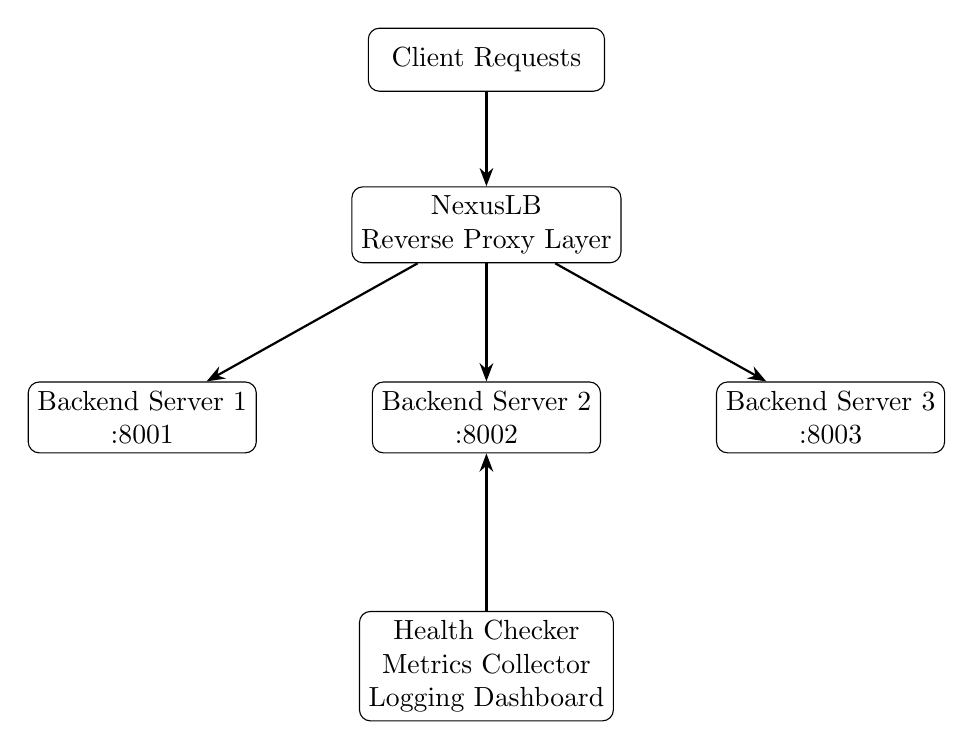
\begin{tikzpicture}[
    node distance=1.2cm and 1.5cm,
    box/.style={
        rectangle,
        rounded corners,
        draw,
        align=center,
        minimum width=3cm,
        minimum height=0.8cm
    },
    backend/.style={
        rectangle,
        rounded corners,
        draw,
        align=center,
        minimum width=2.2cm,
        minimum height=0.8cm
    },
    arrow/.style={
        thick,
        -{Stealth}
    }
]

% Main nodes
\node[box] (client) {Client Requests};

\node[box, below=of client] (nexus) {
    NexusLB\\
    Reverse Proxy Layer
};

% Backend nodes
\node[backend, below left=1.5cm and 1.2cm of nexus] (b1) {
    Backend Server 1\\
    :8001
};

\node[backend, below=1.5cm of nexus] (b2) {
    Backend Server 2\\
    :8002
};

\node[backend, below right=1.5cm and 1.2cm of nexus] (b3) {
    Backend Server 3\\
    :8003
};

% Monitoring node
\node[box, below=2cm of b2] (monitor) {
    Health Checker\\
    Metrics Collector\\
    Logging Dashboard
};


% Arrows
\draw[arrow] (client) -- (nexus);

\draw[arrow] (nexus) -- (b1);
\draw[arrow] (nexus) -- (b2);
\draw[arrow] (nexus) -- (b3);

\draw[arrow] (monitor) -- (b2);

\end{tikzpicture}

\caption{High-level architecture of NexusLB showing client interaction, reverse proxy layer, backend servers, and monitoring components.}

\label{fig:nexuslb_architecture}

\end{figure}

\subsection{Core Workflow}

The core workflow of NexusLB follows a complete request lifecycle from receiving a client request to updating system metrics:

\begin{enumerate}
    \item A client sends an HTTP request to NexusLB, which acts as the single entry point for all incoming traffic.

    \item The request passes through the rate limiting layer to verify whether the client is within the allowed request threshold. Requests exceeding the limit are rejected.

    \item NexusLB checks the backend registry to identify currently available and healthy backend servers.

    \item The load balancing engine applies the selected routing strategy (Round Robin, Least Connections, or IP Hash) to choose the most suitable backend.

    \item The reverse proxy forwards the request to the selected backend server and waits for the response within the configured timeout limits.

    \item If the backend successfully responds, the response is returned to the client. In case of failure, the reliability layer attempts a controlled retry on another healthy backend where applicable.

    \item After completing the request, NexusLB updates system metrics and generates structured logs containing request details, backend information, latency, and response status.

    \item The collected information is displayed through the monitoring dashboard, providing real-time visibility into system performance and backend health.
\end{enumerate}


\subsection{Operational Constraints}

The project is designed with the following operational constraints:

\begin{itemize}
    \item \textbf{Controlled development environment:} NexusLB will initially operate with locally hosted backend servers to allow controlled testing of routing decisions, failures, and performance behaviour.

    \item \textbf{Lightweight implementation:} The system will focus on understanding and implementing core distributed system concepts without depending on complex external infrastructure or managed cloud services.

    \item \textbf{Open-source technology stack:} The implementation will rely on freely available technologies such as Go, Git, GitHub, and Docker to maintain accessibility and reproducibility.

    \item \textbf{Focus on reliability and observability:} The primary objective is to demonstrate correct request handling, failure recovery, and system monitoring rather than achieving production-level performance comparable to enterprise solutions.

    \item \textbf{Single-instance deployment:} The initial version will run as a single NexusLB instance managing a backend pool. Distributed deployment of multiple load balancer instances will be considered as future scope.
\end{itemize}

\section{Solution Approach %
\BvrHint{\ldots engineering focus}}

This project follows an engineering-focused approach where the emphasis is on designing, implementing, and evaluating a reliable distributed traffic management system. The focus is on building a scalable and measurable software component rather than developing novel algorithms. The system will be developed incrementally, with each major module tested independently before integration.

\begin{figure}[ht]
\centering

\resizebox{0.65\textwidth}{!}{
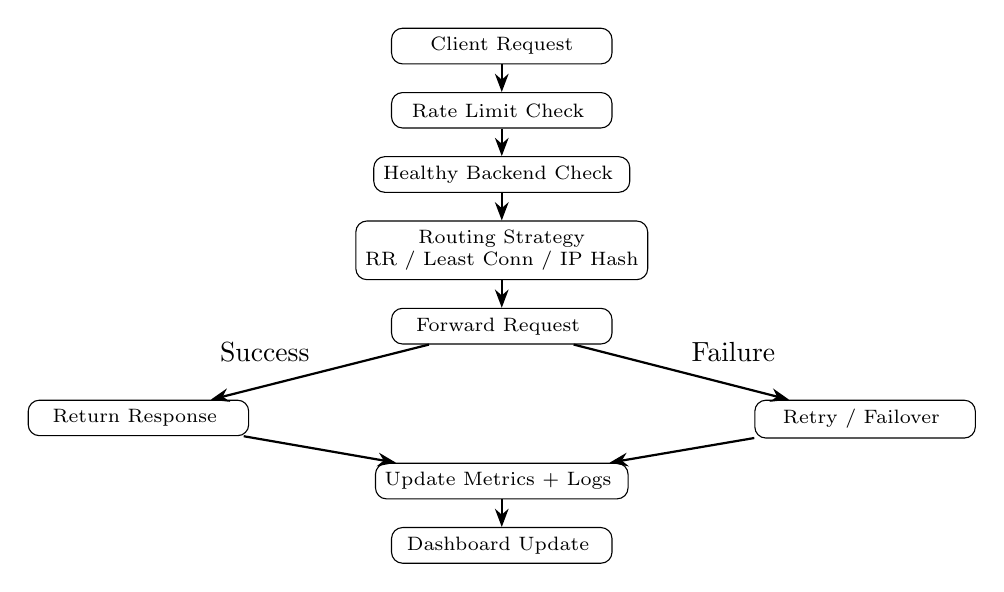
\begin{tikzpicture}[
    box/.style={
        rectangle,
        rounded corners,
        draw,
        minimum width=2.8cm,
        minimum height=0.45cm,
        align=center,
        font=\scriptsize
    },
    arrow/.style={
        thick,
        -{Stealth}
    }
]

% Main flow

\node[box] (request) {Client Request};

\node[box, below=0.35cm of request] (rate) {
Rate Limit Check
};

\node[box, below=0.35cm of rate] (health) {
Healthy Backend Check
};

\node[box, below=0.35cm of health] (strategy) {
Routing Strategy\\
RR / Least Conn / IP Hash
};

\node[box, below=0.35cm of strategy] (forward) {
Forward Request
};


% Branches

\node[box, below left=0.7cm and 1.8cm of forward] (success) {
Return Response
};

\node[box, below right=0.7cm and 1.8cm of forward] (failure) {
Retry / Failover
};


% Merge

\node[box, below=1.5cm of forward] (metrics) {
Update Metrics + Logs
};

\node[box, below=0.35cm of metrics] (dashboard) {
Dashboard Update
};


% Arrows

\draw[arrow] (request)--(rate);
\draw[arrow] (rate)--(health);
\draw[arrow] (health)--(strategy);
\draw[arrow] (strategy)--(forward);

\draw[arrow] (forward)--node[above left]{Success}(success);
\draw[arrow] (forward)--node[above right]{Failure}(failure);

\draw[arrow] (success)--(metrics);
\draw[arrow] (failure)--(metrics);

\draw[arrow] (metrics)--(dashboard);

\end{tikzpicture}
}

\caption{Request lifecycle inside NexusLB showing routing, failure handling, and monitoring updates.}
\label{fig:nexuslb_request_flow}

\end{figure}

\subsection{Load Balancing Strategy Implementation}

The routing logic will be implemented using multiple well-known load balancing strategies rather than relying on a single fixed approach.

\begin{itemize}
    \item \textbf{Strategy-based architecture:} A common load balancing interface will be designed, allowing different routing algorithms to be implemented and replaced without affecting the rest of the system.

    \item \textbf{Multiple routing algorithms:} Round Robin, Least Connections, and IP Hash strategies will be implemented and evaluated based on their request distribution behaviour.

    \item \textbf{Configurable routing behaviour:} The active strategy will be controlled through configuration files, allowing changes without modifying the source code.
\end{itemize}


\subsection{System Architecture}

NexusLB will follow a modular architecture where each responsibility is separated into independent components.

\begin{itemize}
    \item \textbf{Proxy Engine:} Handles incoming HTTP requests and forwards them to selected backend servers.

    \item \textbf{Backend Management:} Maintains the backend server registry and tracks server availability and connection information.

    \item \textbf{Reliability Layer:} Implements health checks, timeout handling, retries, and failover mechanisms to maintain service availability during failures.

    \item \textbf{Observability Layer:} Collects metrics, generates structured logs, and provides dashboard-based monitoring of system behaviour.
\end{itemize}


\subsection{Concurrency and Request Handling}

Since a load balancer must handle multiple requests simultaneously, concurrency will be a core implementation consideration.

\begin{itemize}
    \item Incoming client connections will be handled concurrently using Go routines.

    \item Background processes such as health checks and metrics collection will run independently.

    \item Shared resources such as backend states, connection counts, and collected metrics will be protected using appropriate synchronization mechanisms to prevent race conditions.
\end{itemize}

\begin{figure}[ht]
\centering

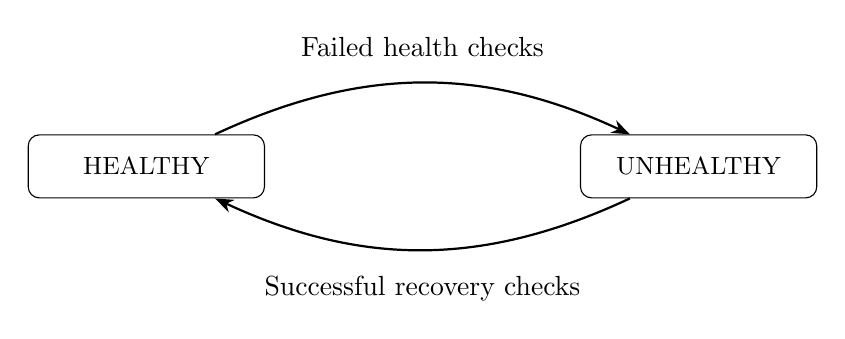
\begin{tikzpicture}[
    state/.style={
        rectangle,
        rounded corners,
        draw,
        minimum width=3cm,
        minimum height=0.8cm,
        align=center,
        font=\small
    },
    arrow/.style={
        thick,
        -{Stealth}
    }
]

\node[state] (healthy) {HEALTHY};

\node[state, right=4cm of healthy] (unhealthy) {UNHEALTHY};


\draw[arrow]
(healthy) to[bend left=25]
node[midway, above=6pt]{Failed health checks}
(unhealthy);


\draw[arrow]
(unhealthy) to[bend left=25]
node[midway, below=6pt]{Successful recovery checks}
(healthy);


\end{tikzpicture}

\caption{Backend health state transition used by NexusLB for failure detection and recovery.}

\label{fig:backend_health_state}

\end{figure}

\subsection{Testing and Performance Evaluation}

The system will be validated through controlled experiments that measure both normal operation and failure handling capabilities.

\begin{itemize}
    \item Test individual components such as routing strategies, health state transitions, rate limiting, and retry logic independently.

    \item Perform integration testing using multiple simulated backend servers connected through NexusLB.

    \item Evaluate system behaviour during backend failures, slow responses, and sudden traffic spikes.

    \item Measure performance indicators such as throughput, latency, error rate, request distribution, and recovery time.
\end{itemize}


\subsection{CI/CD and Incremental Delivery}

Development will follow an incremental delivery approach to ensure that each stage produces a working system component.

\begin{itemize}
    \item Maintain version control using Git and GitHub with regular commits for each implemented module.

    \item Use automated testing to verify system correctness after changes.

    \item Gradually integrate advanced features such as health monitoring, failover handling, metrics collection, and dashboard visualization after the core proxy functionality is stable.
\end{itemize}

\section{Evaluation Criterion %
\BvrHint{\ldots measurable and attributable}}

The success of NexusLB will be evaluated using measurable performance, reliability, and observability metrics directly related to the core system objectives. The evaluation will focus on how effectively the system distributes traffic, handles failures, and maintains visibility into backend behaviour.


\subsection{Primary evaluation metric}

\textbf{Request handling efficiency:} The primary evaluation metric will measure how effectively NexusLB manages incoming requests across multiple backend servers while maintaining acceptable latency and throughput.

\begin{itemize}
    \item \textbf{Target:} Demonstrate efficient request distribution with measurable improvements in backend utilization compared to direct client-to-server communication.

    \item \textbf{Attribution:} Measured using load-testing results, including request distribution across servers, throughput, response latency, and successful request percentage.
\end{itemize}


\subsection{Secondary evaluation metrics}

\begin{itemize}
    \item \textbf{Load distribution accuracy:} Measure how evenly incoming requests are distributed among backend servers under different routing strategies such as Round Robin, Least Connections, and IP Hash.

    \item \textbf{Failure detection and recovery time:} Evaluate how quickly NexusLB detects an unhealthy backend, removes it from routing, and restores it after recovery.

    \item \textbf{Latency and throughput:} Measure average response time, percentile latency (P95/P99), and requests handled per second under different traffic conditions.

    \item \textbf{Fault tolerance:} Evaluate system behaviour during backend crashes, slow responses, and network failures by measuring failed requests, successful retries, and service continuity.

    \item \textbf{Observability quality:} Assess whether collected metrics and structured logs accurately represent request flow, backend health, errors, and system performance.
\end{itemize}


\subsection{Validation plan}

\begin{itemize}
    \item Deploy multiple simulated backend servers and generate controlled client traffic through NexusLB.

    \item Compare different routing strategies by analysing request distribution and performance characteristics.

    \item Perform controlled failure experiments by stopping backend servers, introducing delays, and generating traffic spikes.

    \item Record system metrics such as throughput, latency, error rate, recovery time, and backend health transitions to validate the effectiveness of the implementation.
\end{itemize}

\section{Scalability %
\BvrHint{\ldots with foresight}}

NexusLB is designed with scalability considerations at both the request-handling and system architecture levels. Although the initial implementation focuses on a single load balancer instance managing a controlled backend pool, the modular design allows future expansion.

\begin{itemize}
    \item \textbf{Backend scalability:} The backend registry is designed to support multiple backend servers, allowing additional servers to be added or removed through configuration rather than requiring changes to the core implementation.

    \item \textbf{Algorithm scalability:} The strategy-based load balancing design allows new routing approaches, such as weighted load balancing or latency-aware routing, to be introduced without modifying existing components.

    \item \textbf{Traffic scalability:} Concurrent request handling using Go routines allows NexusLB to process multiple client connections simultaneously while maintaining shared state safely.

    \item \textbf{Future distributed scaling:} A future version could support multiple NexusLB instances working together. However, this introduces additional challenges such as distributed configuration management, shared rate limiting, and centralized monitoring, which are outside the scope of the current implementation.
\end{itemize}

\section{Engineering Available Heuristic}

The project follows established engineering practices and existing infrastructure concepts rather than attempting to develop new load balancing algorithms. The objective is to understand, implement, and evaluate proven techniques used in real-world systems.

\begin{itemize}
    \item \textbf{Existing routing strategies:} Well-known algorithms such as Round Robin, Least Connections, and IP Hash will be implemented and compared instead of designing new balancing algorithms.

    \item \textbf{Incremental development:} The system will be developed in stages, starting with basic request forwarding and gradually adding routing strategies, health monitoring, reliability mechanisms, and observability features.

    \item \textbf{Modular engineering approach:} Components such as proxy handling, backend management, health checks, metrics collection, and logging will remain independent to simplify testing and future improvements.

    \item \textbf{Practical validation:} System behaviour will be evaluated through controlled experiments and measurable benchmarks rather than theoretical assumptions.
\end{itemize}

\section{Project scope and deliverables %
\BvrHint{\ldots iteration-friendly}}

The project scope focuses on developing a functional reverse proxy and load balancer with intelligent routing, reliability mechanisms, and system observability. Development will follow an incremental approach, where the core traffic management functionality is implemented first, followed by advanced monitoring and reliability features.


\subsection{Initial deliverable}

The first iteration will focus on establishing the core functionality of NexusLB:

\begin{itemize}
    \item \textbf{Basic reverse proxy:} Implement an HTTP proxy capable of receiving client requests, forwarding them to backend servers, and returning responses.

    \item \textbf{Backend server management:} Create a backend registry to maintain information about available servers and their current health status.

    \item \textbf{Round Robin load balancing:} Implement the first routing strategy to distribute incoming requests across multiple backend servers.

    \item \textbf{Configurable backend setup:} Support defining backend servers and basic system settings through a configuration file.

    \item \textbf{Unit testing and validation:} Test core components such as request forwarding, backend selection, and configuration handling.

    \item \textbf{Version control and development workflow:} Maintain the project repository with structured commits and incremental feature integration.
\end{itemize}


\subsection{Subsequent deliverables}

Later iterations will extend the system with reliability, performance, and monitoring capabilities:

\begin{itemize}
    \item \textbf{Advanced routing strategies:} Implement Least Connections and IP Hash algorithms and compare their performance under different workloads.

    \item \textbf{Health monitoring and failover:} Add periodic health checks, automatic removal of unhealthy backends, and recovery-based reintegration.

    \item \textbf{Reliability mechanisms:} Implement request timeouts, controlled retries, and failover handling for backend failures.

    \item \textbf{Traffic control features:} Introduce rate limiting to protect backend services during sudden traffic increases.

    \item \textbf{Metrics and dashboard:} Develop monitoring capabilities to display request rate, latency, error rate, backend health, and traffic distribution.

    \item \textbf{Structured logging and tracing:} Add detailed request logs containing request identifiers, backend information, response status, and processing time.

    \item \textbf{Benchmarking and evaluation:} Conduct experiments measuring throughput, latency, failure recovery time, and routing behaviour.
\end{itemize}

\section{Risks and Mitigations}

\begin{itemize}

    \item \textbf{Concurrency and synchronization issues:} Multiple client requests, health checks, and metrics collection running simultaneously may introduce race conditions or inconsistent system states.  
    \textbf{Mitigation:} Design shared components carefully and use synchronization mechanisms such as mutexes or atomic operations. Test concurrent behaviour early using controlled workloads.

    \item \textbf{Scope expansion:} Implementing a complete production-grade load balancer involves several advanced features beyond the semester timeline.  
    \textbf{Mitigation:} Prioritize the core MVP consisting of reverse proxy functionality, routing strategies, health checks, and fault handling. Advanced features such as distributed deployment will remain future scope.

    \item \textbf{Performance measurement variability:} Benchmark results may vary depending on hardware limitations, system background processes, and test conditions.  
    \textbf{Mitigation:} Keep testing conditions consistent, repeat experiments multiple times, and report measured results rather than assumed performance values.

    \item \textbf{Failure handling complexity:} Retry and failover mechanisms may introduce unexpected behaviour, especially for requests that are not safe to repeat.  
    \textbf{Mitigation:} Implement controlled retries with clear limitations and evaluate failure scenarios carefully before enabling automatic recovery.

    \item \textbf{Dashboard development affecting core progress:} Building monitoring and visualization features may consume time needed for the main backend implementation.  
    \textbf{Mitigation:} Develop the dashboard only after the core routing and reliability components are stable, using already available metrics APIs.

    \item \textbf{Security limitations:} Features such as TLS termination and request validation may not provide production-level security without extensive auditing.  
    \textbf{Mitigation:} Clearly define the project as an educational implementation focused on infrastructure concepts rather than a production replacement for systems like NGINX or HAProxy.

\end{itemize}


\section{Summary}

This project proposes the development of NexusLB, a custom reverse proxy and load balancer designed to improve traffic management, reliability, and observability in distributed web applications. The system focuses on intelligent request routing, health-aware backend management, fault tolerance, and real-time monitoring through a modular engineering approach.

The project emphasizes measurable evaluation through controlled experiments involving routing performance, failure recovery, latency, throughput, and system behaviour under different workloads. By implementing established infrastructure concepts such as load balancing strategies, health checks, retries, and metrics collection, NexusLB aims to provide practical understanding of how modern distributed systems handle scalability and reliability challenges.

The project remains focused on engineering implementation and evaluation rather than developing novel algorithms. Its contribution lies in building a functional, measurable, and extensible infrastructure component that demonstrates the principles behind real-world traffic management systems.

\end{document}